\section{RxJS: Reactive Extensions For JavaScript}
Rx ist eine Library, die für zahlreiche Programmiersprachen zur Verfügung gestellt wird. Diese finden sowohl in der Frontend als auch in der Backend-Implementierung Anwendung. In dieser Arbeit wird der Fokus auf RxJS geworfen. Diese Library ist eine Erweiterung speziell für Javascript/Typescript. RxJS erlaubt es mit Hilfe von Observable-Sequenzen Event-basierte Programme zu erstellen. Dabei wird dieser Ansatz auch als \textbf{reactive Programming} definiert. Neben der Kernfunktionalität von Observables werden auch Subjects und Schedulers geboten. Sollte man von reactive Programming noch nichts gehört haben, dann wird die größte Herausforderung sein \glqq{}reactive\grqq{} zu denken.

\subsection{Reactive Programming}
Im Kern ist reactive Programming ein Programmierparadigma. Im \textbf{reaktiven Manifest}, zu finden unter

\begin{center}
\url{https://www.reactivemanifesto.org/de},
\end{center}

\noindent
wird bereits beschrieben, dass Reactive Programming als Programmierung mit asynchronen, unveränderlichen Streams von Events bezeichnet wird. Laut der offiziellen Dokumentation richtet sich ReactiveX nach dem Beobachter-Muster (engl. Observer-Pattern). Das Observer-Pattern ist ein Entwurfsmuster, in der Änderungen eines Objektes (Subjects genannt) an einer Liste abhängiger Strukturen weitergereicht wird. Diese abhängige Strukturen (Observers) werden bei jeder Zustandsveränderung informiert. Eine Veränderung eines Objekts kann hierbei gleichgesetzt werden mit neuen Wert innerhalb eines Datenflusses. Als Beispiel für eine reaktive Anwendung kann Excel genommen werden. Ändert man einen Wert in einer Zelle, ändert sich auch der Wert in der Summenzelle. Die Zelle, deren Wert geändert wurde, löst ein Event aus, den die Summen-Zelle empfängt. Daraufhin findet eine Neuberechnung statt.\cite{reactive-programming-beispiel} Datenflüsse können aus verschiedensten Operationen entstehen wie z.B. Klick-Events, Variablen, Cache etc. Als Observer kann man sich in diesem Datenfluss einhängen und entsprechend reagieren.\cite{rx-intro} Rx bietet eine enorme Menge an Funktionen diese Datenflüsse zu bearbeiten/manipulieren (siehe Sektion Operatoren). Diese Operatoren komplett abzudecken wird in dieser Arbeit unmöglich sein, jedoch wird nach dem behandeln dieses Kapitels ein gewisses Grundverständnis für neue Operatoren entstehen und wie diese in Folge anzuwenden sind. Die grundlegenden Konzepte, um asynchrone Events in RxJS zu steuern, sind:

\begin{itemize}
    \item Observable: Repräsentiert die Idee einer abrufbaren Sammlung, in der zukünftige Werte oder Events gelagert sind.
    \item Observer: Eine Sammlung von Callbacks die, die  aus dem Observable-Stream gelieferten Werte, abrufen.
    \item Subscription: Repräsentiert das Aufrufen eines Observable.
    \item Operators: Funktionen, die das Verhalten von Observable-Streams beeinflussen.
    \item Subjects: Eventgeneratoren, die Events an zuhörende Observer zurückgibt. Im Gegensatz zu Observables, sind Subjects standardmäßig multicasting fähig.
    \item Schedulers: Steuerungsmechanismen die bestimmen, wann eine Subscription startet und wann Werte aus dem Stream an die Observer übermittelt werden.
\end{itemize}

\subsection{Observables}

Observables sind eine träge Sammlung von multiplen Werten. Sie füllen den fehlenden Platz in der unten stehenden Tabelle:

\begin{center}
    \begin{tabular}{| l | l | l |}
    \hline
    & \textbf{Einzelne-} & \textbf{Multiple Werte} \\ \hline
    \textbf{Pull/synchron} & Funktionen & Iterables (Arrays, Strings, ...) \\ \hline
    \textbf{Push/asynchron} & Promises & Observables  \\ \hline
    \end{tabular}
\end{center}

\noindent
Das Push- und Pull-Prinzip beschreibt dabei wie ein Datenproduzent mit dem Datenverarbeiter kommuniziert. In \textbf{Pull-Systemen} bestimmt der Verarbeiter, wann die Daten vom Ersteller angenommen werden. Der Ersteller selbst weiß nicht wann die Daten angefragt werden. Jede Javascript Funktion unterliegt einem Pull-System. Die Funktion ist ein Verarbeiter von Daten und diese kann im Code jederzeit abgerufen werden.\\

\noindent
Das \textbf{Push-Prinzip} wird im nächsten Beispiel deutlich. Vor dem Ausführen des Beispiels muss ../rxjs/introduction.ts als Eingangsdatei definiert werden.

\begin{figure}[H]
\begin{lstlisting}[basicstyle=\small]
const alias: Observable<number> = RxJS.Observable.create((observer) => {
    observer.next(1);
    observer.next(2);
    observer.next(3);
    setTimeout(() => {
        observer.next(4);
        observer.complete();
    }, 1000);
});

console.log('Before subscribe');
alias.subscribe({
    next: x => console.log('Value: ' + x),
    error: err => console.error('Error occurred: ' + err),
    complete: () => console.log('Done!'),
});
console.log('After subscribe');
\end{lstlisting}
\caption{Observable verhalten sich sowohl synchron als auch asynchron.}
\end{figure}

\noindent
Das Observable-Objekt repräsentiert eine Kollektion die Werte zu seinen Beobachtern liefert. In diesem Beispiel wird ein Observable erstellt, dass sofort (synchron) die Werte 1, 2 und 3 produziert, sobald die Subscription gestartet wird. Der vierte Wert wird asynchron übermittelt und das Observable daraufhin geschlossen. Wichtig ist, dass man sich ein Observable-Stream nur mit der subscribe()-Methode anschließen kann. Die Konsole gibt die Werte in folgender Reihenfolge aus:

\begin{figure}[H]
\begin{center}
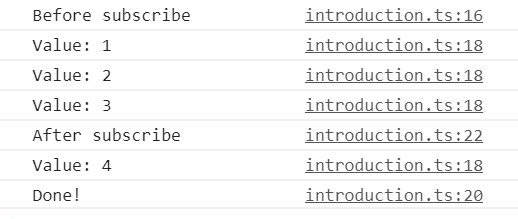
\includegraphics{observable-create-console}
\end{center}
\end{figure}

\noindent
Bei einer Subscription können drei verschiedene Events auftreten und somit drei verschiedene Funktionen aufgerufen werden:

\begin{itemize}
\item next: () =\textgreater Wenn ein Wert ausgegeben wird,
\item error: () =\textgreater Wenn ein Fehler ausgegeben wird,
\item complete: () =\textgreater Wenn sich der Stream schließt.
\end{itemize}

\noindent
In Push-Systemen steuert der Datenproduzent, wann die Daten an die Zu-hörenden übermittelt werden. Der Datenverarbeiter weiß hingegen nicht, wann die Daten ankommen. Promises sind ein typisches Beispiel für Push-Systeme. Ein Promise (Produzent) übermittelt einen eingetroffenen Wert an angeschlossene Callbacks (Verarbeiter). Ungleich wie mit Funktionen bestimmen Promises, wann die Werte an die Callbacks weitergereicht wird. Observables zählen zu einem neuen Push-System in Javascript. Im Gegensatz zu Promises emittieren Observables multiple Werte in Form von Streams. Zur Unterscheidung:

\begin{itemize}
\item Eine Funktion ist eine träge ausführende Operation, die beim Abruf ein Wert synchron zurückgibt.
\item Ein Promise ist eine Operation die einen eventuell eintreffenden oder nicht-eintreffenden Wert zurückgibt.
\item Ein Observable ist eine träge ausführende Operation, dass synchron oder asynchron keine oder potenziell unendlich viele Werte ab dem Zeitpunkt des Aufrufs zurückgibt.
\end{itemize}

\noindent
Hierbei stellt sich die Frage, was bedeutet träge? Träge Funktionen, im englischen auch als \textit{lazy Functions} bezeichnet, sind Funktionen die erst bei ihrem Aufruf Werte produzieren.\cite{lazy-functions}

\begin{figure}[H]
\begin{lstlisting}[basicstyle=\small]
function foo() {
    console.log('Hello');
    return 42;
}

const x = foo.call(this); // same as foo()
console.log(x);
const y = foo.call(this); // same as foo()
console.log(y);
\end{lstlisting}
\end{figure}

\begin{figure}[H]
\begin{lstlisting}[basicstyle=\small]
const foo = Rx.Observable.create((observer) => {
  console.log('Hello');
  observer.next(42);
});

foo.subscribe((x) => {
  console.log(x);
});
foo.subscribe((y) => {
  console.log(y);
});
\end{lstlisting}
\end{figure}

\noindent
Der Output bleibt immer derselbe:

\begin{figure}[H]
\begin{center}
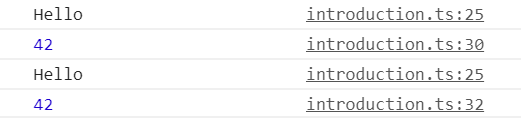
\includegraphics{observable-lazy-console}
\end{center}
\end{figure}

\noindent
Das liegt daran, da sowohl Funktionen als auch Observables träge sind. Die Operationen innerhalb beider Typen findet erst beim Aufruf statt. Mit anderen Worten: Das starten einer Subscription ist analog zum Aufruf einer Funktion. Entgegen der Annahme, dass Observables ausschließlich asynchron operieren, können diese ebenfalls synchron Werte ausgeben (siehe Abb. 22).
Der Hauptpunkt in dem Observables sich von Funktionen unterscheiden ist, dass Observables mehrere Werte (mit der Zeit) emittieren können. Innerhalb einer Funktion ist es nicht Möglich zwei return Ausdrücke einzubauen, die zusammen ausgegeben werden.

\subsubsection{Anatomie eines Observable}
Observables werden entweder mit der create Methode, mit einer Observable-Instanz oder mit der Hilfe eines Observable-Operators \textbf{erstellt}. Der Datenfluss wird an den Observern mit der subscribe()-Methode \textbf{überreicht}. Letzteres kann eine Subscription \textbf{abgesetzt} werden.

\subsubsection{Observables erstellen}

\begin{figure}[H]
\begin{lstlisting}[basicstyle=\small]
const randomNumber = new Observable<number>(observer => {
    observer.next(Math.random());
});
\end{lstlisting}
\caption{Instantiierung eines Observables, als Parameter wird ein Callback angenommen.}
\end{figure}

\noindent
Die statische Methode Observable.create() ist ein alias ist zum Konstruktor-Aufruf. Für gewöhnlich werden jedoch sog. \textit{creation operators} wie \textbf{of}, \textbf{from}, \textbf{interval} etc. angewendet, um Observables zu erstellen. Im nächsten Abschnitt werden die verschiedenen Observable-Typen gegenübergestellt.

\subsubsection{Datenfluss überreichen}

Beim Aufruf der subscribe()-Methode überreicht der Datenproduzent ein eigenständigen Datenfluss an die Observer. Das hat zur Folge, dass mehrere Observer sich dem gleichen Observable anschließen und dennoch unterschiedliche Werte bekommen können.

\begin{figure}[H]
\begin{lstlisting}[basicstyle=\small]
const randomNumber = new Observable<number>(observer => {
    observer.next(Math.random());
});

randomNumber.subscribe(value =>
    console.log('1st subscription emits: ', value));
randomNumber.subscribe(value =>
    console.log('2nd subscription emits: ', value));
\end{lstlisting}
\end{figure}

\begin{figure}[H]
\begin{center}
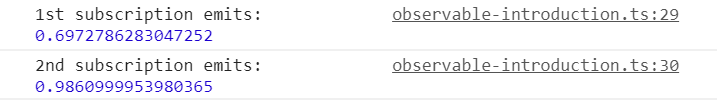
\includegraphics[width=12cm]{unicasting-observables}
\end{center}
\end{figure}

\noindent
Das Ergebnis sind zwei verschiedene Werte, bei zwei Subscriptions an einem Observable. Diese Eigenschaft wird als \textbf{unicasting} bezeichnet. Das ist nur Möglich, da die Funktion random() erst dann aufgerufen wird, wenn ein Observable mit der subscribe()-Methode aufgerufen wird. Somit hat jede Subscription einen eigenen Datenproduzent. Es gibt nun mehrere Möglichkeiten, dass sich Observers den gleichen Datenfluss teilen. Eine Möglichkeit wäre, den Datenproduzent außerhalb des Observable auszulagern. 

\begin{figure}[H]
\begin{lstlisting}[basicstyle=\small]
const dataProducer: number = Math.random();
const randomNumber = new Observable<number>(observer => {
    observer.next(dataProducer);
});

...
\end{lstlisting}
\end{figure}

\noindent
Eine elegantere Variante, wäre ein Operator anzuwenden, der den zuletzt eingetretenen Wert an die verschiedenen Observer teilt:

\begin{figure}[H]
\begin{lstlisting}[basicstyle=\small]
const multicast = randomNumber.pipe(shareReplay());

multicast.subscribe(value =>
    console.log('1st subscription emits: ', value));
multicast.subscribe(value =>
    console.log('2nd subscription emits: ', value));
\end{lstlisting}
\end{figure}

\noindent
Nun können multiple Subscriptions am Observable die gleiche Sequenz empfangen, da shareReplay() dafür sorgt, dass der Datenproduzent nur einmal aufgerufen werden kann und weitere Subscriptions sich diesen Datenproduzenten teilen. Diese Eigenschaft wird auch als \textbf{multicasting} bezeichnet. Das Ergebnis sieht wie folgt aus:

\begin{figure}[H]
\begin{center}
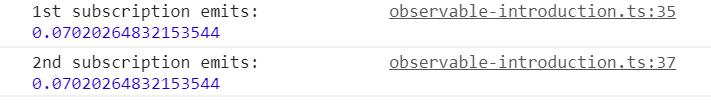
\includegraphics[width=12cm]{multicasting-observables}
\end{center}
\end{figure}

\noindent
Wenn Werte eines Streams erst beim Aufruf einer Subscription entstehen, handelt es sich hierbei um \textbf{cold Observables}.\cite{hot-vs-cold} Dies ist in jedem der oben angeführten Beispielen der Fall. Um auf die oben angeführte These zurück-zukommen, dass Observables träge sind, war dies zwar zum Einstieg in die Thematik hilfreich, aber nur die halbe Wahrheit. Observables können Werte emittieren auch ohne der subscribe()-Methode. Das bedeutet es werden Werte ausgestoßen, unabhängig davon ob eine Subscription stattfindet oder nicht. Hierbei würde es sich um ein \textbf{hot Observable} handeln. Um einen besseren Einblick zu bekommen, wird ein Observable erstellt, dass unendlich viele Werte ausstößt.

\begin{figure}[H]
\begin{lstlisting}[basicstyle=\small]
const infinite = RxJS.interval(1000).pipe(publish());
infinite.connect();

setTimeout(() =>
    infinite.subscribe(v => console.log('1st subscriber:', v)), 2000);
setTimeout(() =>
    infinite.subscribe(v => console.log('2nd subscriber: ', v)), 3000);
\end{lstlisting}
\end{figure}

\noindent
Die statische Methode interval() erstellt ein Observable, dass aufsteigend Nummern ausgibt innerhalb eines festgelegten Intervalls. Der Startindex ist 0. Der publish() Operator sorgt dafür, dass das Observable in einem \textbf{connectable Observable} umgewandelt wird. Das heißt es werden erst Werte innerhalb der Sequenz emittiert, sobald die entsprechende connect() Methode am Observable aufgerufen wird. Alle dazugehörigen Observers bekommen, ab dem Zeitpunkt der Subscription die Werte der Quelle überreicht.\\

\begin{figure}[H]
\begin{center}
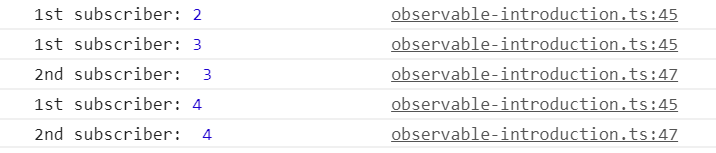
\includegraphics[width=12cm]{hot-observable}
\end{center}
\end{figure}



\noindent
Wie man nun gesehen hat hängt es vom Observable ab, wann die Sequenz von Werten emittiert werden. Ein hot Observable könnte Werte ausstoßen, sobald es erstellt wird. Und deshalb könnten Observers, die sich später am Observable-Stream einhängen, Werte zwischenzeitlich verpassen. Wenn der gleiche Datenproduzent über verschiedene Subscriptions genutzt wird, ist dies ebenfalls ein Indikator dafür, dass es sich um ein hot Observable handeln könnte. Ein cold Observable dagegen wartet mit dem emittieren der Werte, bis eine Subscription eines Observers stattgefunden hat. Dieser Observer empfängt dementsprechend die gesamten Werte der Sequenz. In manchen Versionen von Rx gibt es auch die Bezeichnung connectable Observable. In solchen Fällen werden erst dann Werte emittiert, wenn die dazugehörige connect() Methode aufgerufen wurde, unabhängig davon ob eine Subscription an dem Observable stattfindet oder nicht.\cite{hot-vs-cold-part-2}

\subsubsection{Subscription absetzen}


\noindent
\begin{center}
***Hier fehlt noch ordentlich was.*** 
\end{center}


\subsection{Operatoren}
Wenn es um Operatoren geht, sind diese die wahre Stärke der Observables. Operatoren gibt es in verschiedenen Kategorien: Sie manipulieren das Stream-Verhalten oder bearbeiten die Werte innerhalb eines Streams. Eines haben Operatoren gemeinsam. Wenn ein Operator an einem Stream angewendet wird, wird ein neuer Stream erstellt. Das liegt daran, dass Streams an sich unveränderbar (engl. immutable) sind.
Mit der aktuell neuesten Version von RxJS (6) ist nur noch Möglich Operatoren innerhalb der pipe() Methode anzuwenden.  ....


\subsection{Subjects}
\subsection{Schedulers}









